\documentclass{standalone}
\begin{document}

In our previous progress report, we described an approach where the robot rotated the valve stem by fitting the wrench head onto the shaft, then solving the inverse kinematics (IK) and moving its arm in a circular trajectory constrained to a plane parallel to the panel surface.
Due to joint limits of the robot, the IK for the trajectory may
not be solvable at certain arm positions. To reduce the chance of encountering unsolvable IK, we turned the wrench $90^{\circ}$ at a time, solving for a quarter circle trajectory's IK, and turn the valve stem four times. However, a drawback of this strategy is the time required to
complete the task. Thus, we designed a new gripper that uses the ring
end of the wrench, centered at the axis of rotation of the gripper servo
motor, by aligning and fitting the ring end to the valve
stem, and rotating the valve stem by rotating the gripper motor
$360^{\circ}$. Our new gripper is capable of rotating the valve 
stem with $5Nm$ of torque and complete the task without having
to solve for multiple IK's.

%% The last gripper in task 2 our humanoid robot have to fit the wrench
%% into the shaft and rotate $360$ degrees by move the arm and solve the
%% inverse kinematics. However, sometimes(usually) the inverse kinematics
%% can not be solved due to the limitation of the arm. In the first
%% report we attempt to rotate the wrench $4$ times with $90$ degrees
%% each time. This is very time consuming and now we designed a new
%% gripper that use the servo motor attached to the gripper which can
%% directly robot $360$ degrees and capable of the torque $5Nm$. 


Figure \ref{gripper} illustrates the new gripper which consists of a
servo motor and a magnetic attachment. We use a Dynamixel MX-106
servo motor which has a high stall torque of $8.4Nm$. At a payload of 
$5Nm$, the motor can still rotate at a speed of
more than $10 rpm$, thus, it allows our robot to complete turning 
the valve stem much faster.

%% To pick and align the wrench onto the shaft more reliably, the gripper is equipped with a spring-loaded attachment. When the wrench is picked by the robot, the spring push the central stick inside the ring end of the wrench to
%% ensure perfect alignment. The ring end of the wrench is used to
%% manipulate the shaft. To align the wrench to the shaft, only the
%% central stick needs to be aligned to the shaft. After alignment, the
%% gripper is pushed against the shaft which will result in the spring to
%% compress and the ring end of the wrench pushed into the shaft as shown
%% on the right in Fig.\ref{gripper}. The shaft is then easily rotated
%% using the Dynamixel motor.

%% FUTURE WORK
%% <<<<<<<<<<<<<<<<<
%% We need more experiments to validate the feasibility of
%% this gripper and then we can decide whether to equip this kind of
%% gripper in the final or not.
%% >>>>>>>>>>>>>>>>>>>>

 \begin{figure}%[hb]
    \begin{center}
    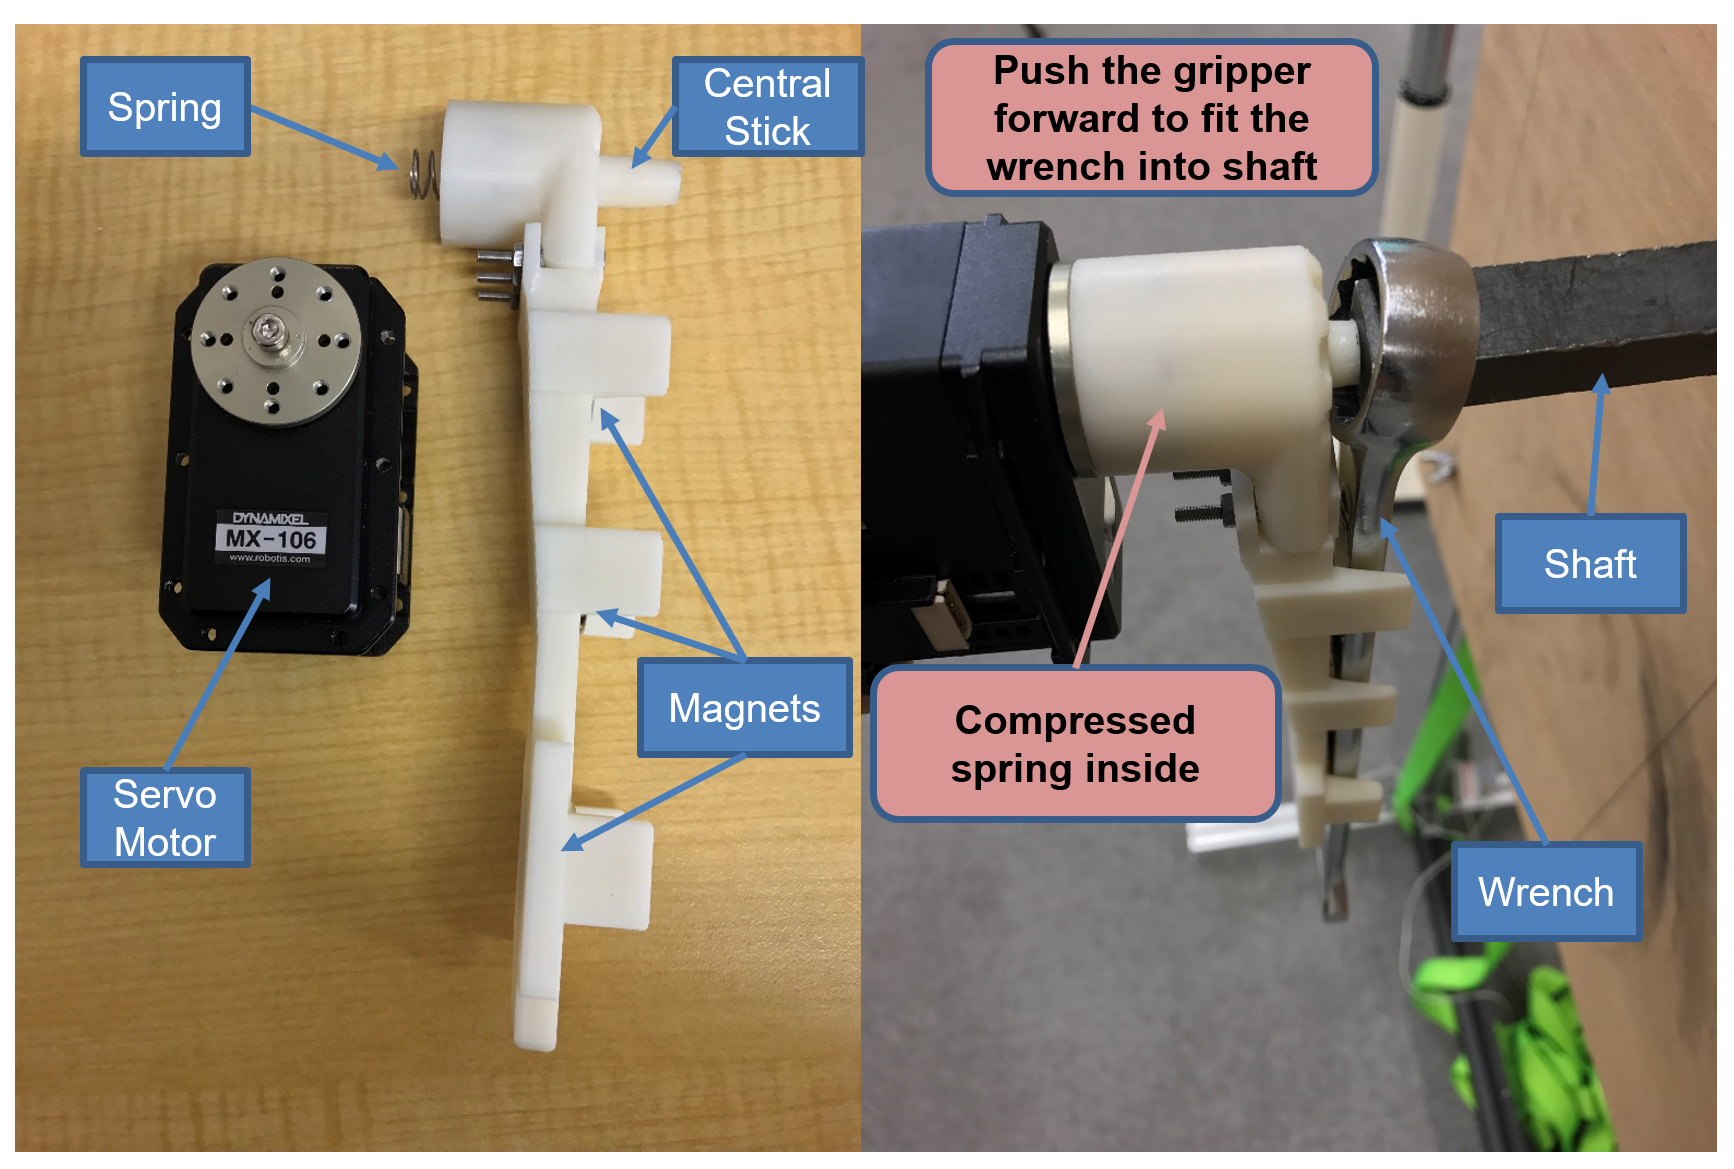
\includegraphics[keepaspectratio=true, width=1\linewidth,
      height=0.3\textheight]{sections//task2//images//gripper.png}
      \end{center}
    \caption{New Gripper Design}
    \label{gripper}
 \end{figure}

\end{document}
